\documentclass{article}
\usepackage[utf8]{inputenc}
\usepackage{hyperref}

\title{Übung 4}
\author{Laurenz Weixlbaumer, 11804751}
\date{November 2018}

\renewcommand\thesubsection{(\alph{subsection})}

\usepackage{enumitem}
\usepackage{mathtools}

\begin{document}

\maketitle

\section{Ansteuerung der Operation \normalsize{(MUX-2 Multiplexer)}}

\begin{enumerate}[label=(\alph*)]

\item Schaltbild eines MUX-2 Multiplexers aufgebaut aus MUX-1 Basisblöcken.

\begin{figure}[htp]
\begin{center}
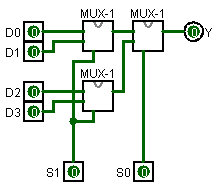
\includegraphics[width=6cm]{mux2_circuit.png}
\end{center}
\end{figure}

\end{enumerate}

\end{document}
